

\section{Problem 3}
\label{part3}
Consider the "bow-tie" graph in the Broder et al. paper (fig 9):
http://www9.org/w9cdrom/160/160.html\\


\noindent Now consider the following graph:
    \begin{verbatim}
    A --> B
    B --> C
    C --> D
    C --> A
    C --> G
    E --> F
    G --> C
    G --> H
    I --> H
    I --> J
    I --> K
    J --> D
    L --> D
    M --> A
    M --> N
    N --> D
    O --> A
    P --> G
     \end{verbatim}
    For the above graph, give the values for:\\
IN: \\
SCC: \\
OUT: \\
Tendrils: \\
Tubes: \\
Disconnected:

\subsection{Solution}

\begin{figure}
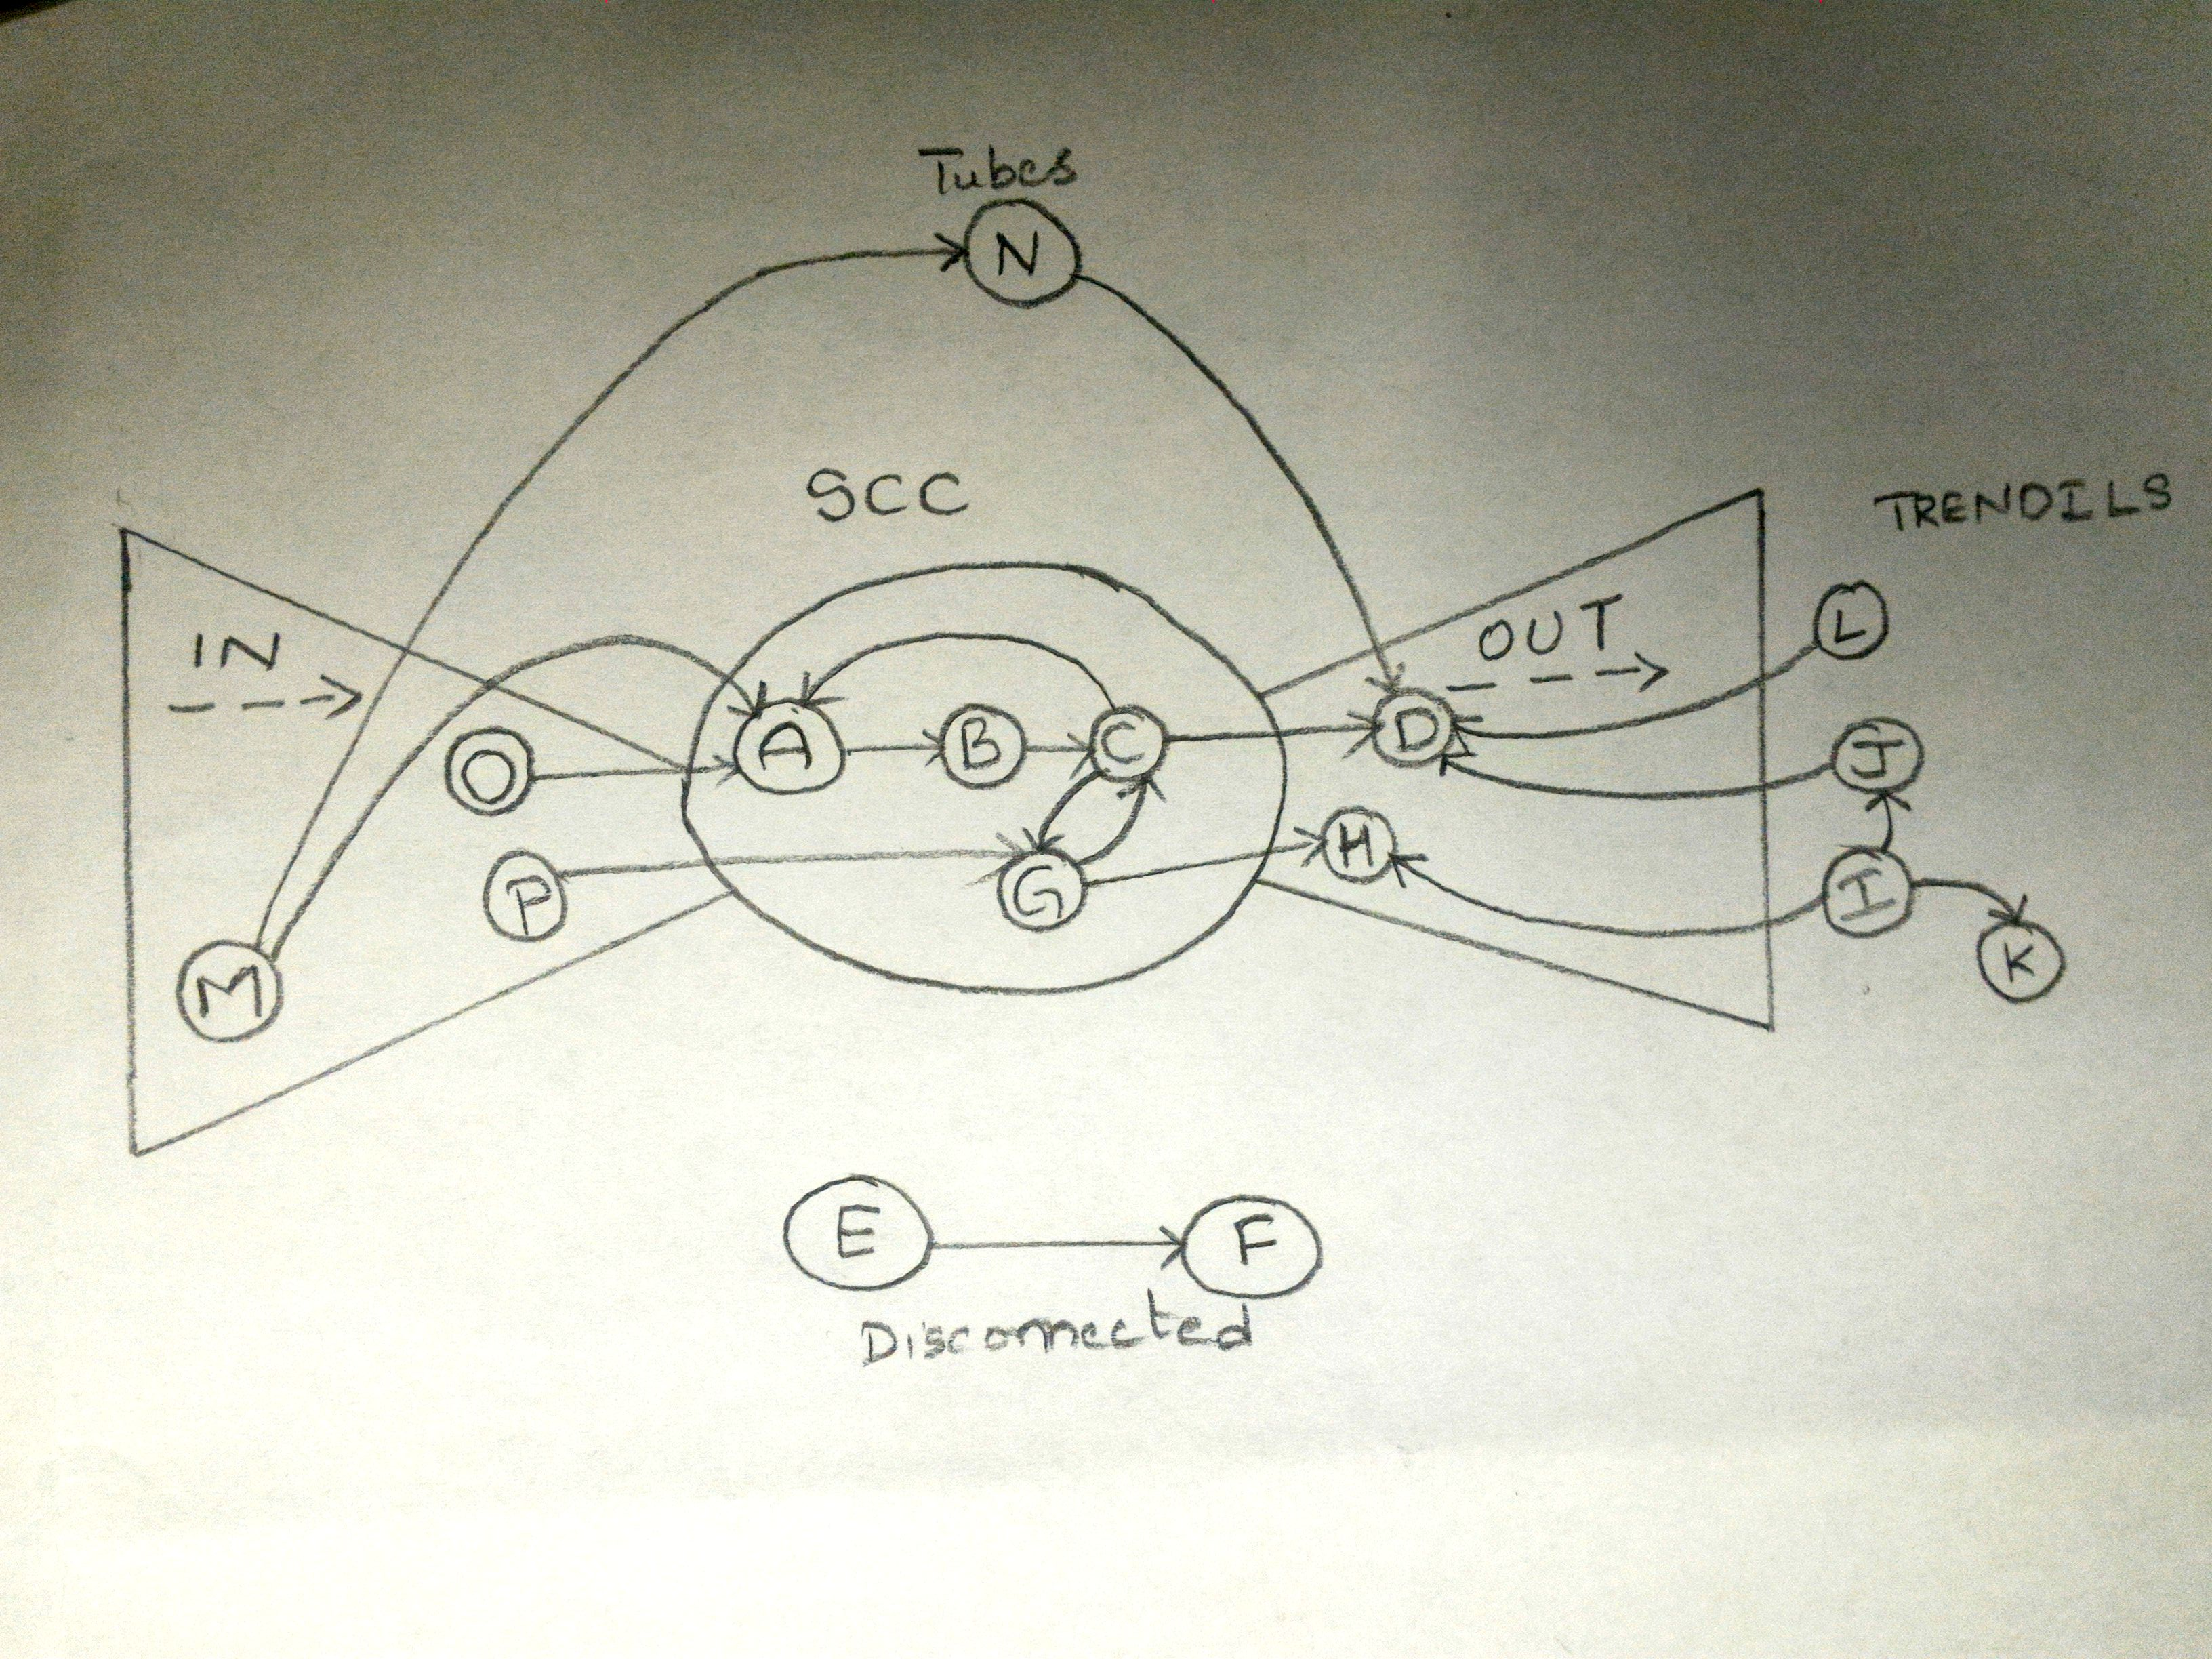
\includegraphics[scale=0.15]{bow-tie.png}
\caption{Drawing of the example graph}
\label{fig:X-distribution}
\end{figure}


Model graph is drawn based on the bow-tie concept including all the node points stated above.

\begin{verbatim}
IN: M,O,P
SCC: A,B,C,G,
OUT: D,H
In Tendril: None
Out Tendril : L,K,I,J
Tubes: N
Disconnected: E,F
\end{verbatim}


Explanations for each node have been provided below.

\textbf{IN:}  $O, M, P$

According to the definition of IN, any node in IN can be connected to any other node in IN or can be connected to any node in SCC but not with any other nodes. $M$,$O$,$P$ falls into this category they are connected to $A$,$G$ nodes in SCC.

\textbf{SCC:}  $A, B, C, G$

Strongly Connected Component consists of group of nodes which are connected to each other directly or indirectly and these nodes can be connected from IN and connected to OUT. $A$,$B$,$C$,$G$ come under this category.

\textbf{OUT:}  $D, H$

Nodes which exit from SCC and are not connected back to SCC come under OUT. $D$ and $H$ show these characteristics so they come under \emph{OUT}.

\textbf{Tendrils:}  $I, J, K, L$

The nodes which cannot be directly connected to the nodes in SCC. $I$,$J$,$K$,$L$ come under \emph{Tendrils}.

\textbf{Tubes:} $N$

Nodes which pass from IN to OUT without any interaction with SCC are called \emph{tubes}. $N$ is a tube linking from $M$ to $D$.

\textbf{Disconnected:}  $E, F$

The Disconnected components link to no one in the graph, and stand alone.  They are not defined explicitly by Broder, et. al, but their meaning is implied within the paper.

\newpage

\begin{thebibliography}{1}
\bibitem{one}
 How to fetch Internet Resources Using urllib2, 
{\tt \\https://docs.python.org/2/howto/urllib2.html}.

\bibitem{two}
Curl,  
{\tt \\http://curl.haxx.se/docs/manpage.html}.

\bibitem{three}
BeautifulSoup Documentation, 
{\tt \\http://www.crummy.com/software/BeautifulSoup/bs4/doc/}.

\bibitem{four}
Stack Overflow answering questions on Content-type, 
{\tt \\http://stackoverflow.com/questions/2143674/how-do-i-get-a-content-type-of-a-file-in-python-with-url}.

\bibitem{five}
Graph Strducture in the Web, 
{\tt \\http://www9.org/w9cdrom/160/160.html }.

\end{thebibliography}
 
 